\documentclass[12pt]{extarticle}
\usepackage{graphicx}
\usepackage{setspace}
\usepackage{xcolor}
\usepackage[a4paper, total={6in, 8in}]{geometry}
\usepackage{pgfgantt}

\begin{document}

\doublespacing

\title{\textbf{Debugging Problems}}
\author{Patrick Farmer\\ Supervisor: Dr. Jonathan Dukes}
\date{\today}
\maketitle

\begin{figure}[h!]
\centering

\includegraphics[width=\linewidth]{Images/Trinity_Main_Logo.jpg}
\label{fig:logo}
\end{figure}

\begin{center}
\large A Dissertation submitted in partial fulfillment of the requirements for the degree of MAI in Computer Engineering.
\end{center}

\newpage
\title {\Huge \textbf{\textcolor{blue}{Declaration}}}

\vspace{0.5cm}
\small I hereby declare that this Dissertation is entirely my own work and that it has not been submitted as an exercise for a degree at this or any other university.

\vspace{0.5cm}
\small I have read and I understand the plagiarism provisions in the General Regulations of the University Calendar for the current year, found at http://www.tcd.ie/calendar.
\vspace{0.5cm}

\small I have completed the Online Tutorial on avoiding plagiarism `Ready Steady Write', located at http://tcd-ie.libguides.com/plagiarism/ready-steady-write.
\vspace{0.5cm}

\small I consent to the examiner retaining a copy of the thesis beyond the examining period, should they so wish (EU GDPR May 2018).
\vspace{0.5cm}

\small I agree that this Dissertation will not be publicly available, but will be available to TCD staff and students in the University’s open access institutional repository on the Trinity domain only, subject to Irish Copyright Legislation and Trinity College Library conditions of use and acknowledgement.
\vspace{2cm}

\small Signed:~Patrick Farmer\hfill Date:~\today

\newpage
\tableofcontents

\newpage
\section{Acronyms}

\begin{itemize}
    \item LLM - Language Model
    \item AST - Abstract Syntax Tree
    \item AI - Artificial Intelligence
    \item API - Application Programming Interface
    \item GPT - Generative Pre-trained Transformer
\end{itemize}

\section{Introduction}

\subsection{Context}

In recent years there have been great strides made in the ability of LLMs to generate code. These LLMs are already being integrated into employee workflows in companies all over the world. This will place a much greater emphasis on the debugging process as the code generated by these LLMs much be inspected and fixed when bugs are produced. It has also been noted in many studies that debugging is an extremely important skill as it is the most difficult part of the programming process and is also the most often overlooked when teaching programming. More will be discussed on this in the literature review. This project will aim to create a tool that will help teach debugging to students who will be the future employees of these companies. 

\subsection{Aims}

The aim of this tool is quite simple. To generate problems for students. The language, code topic and bug type should all be customisable. 

It was also a goal to create two different methods for inserting the bug which can be compared with each other. The first method being to insert the bug by querying the LLM and the second method being to insert the bug by walking through the AST of the code and inserting the bug semi manually.

Another aim of the project was to create test cases that the code could be tested against to ensure that the bug was inserted correctly. These same test cases could then be used by a student to test their solution to the problem.

The creation of a frontend was not a goal of this project, the meaningful work of this project is all done in the backend and a frontend could be added at a later date.

\subsection{Evaluation Metrics}

It was decided early on that the evaluation and measuring of the project success would be done using desktop metrics and that there would not be a user study. The metrics that were decided on were code complexity, code diversity, attempt count and run time. The calculation of these metrics and the reasoning behind them will be discussed in the testing and evaluation section.

\subsection{Structure of the Dissertation}

The structure of the dissertation will be as follows. The background will go through previous work done in the area of debugging and LLMS. It will also give a brief overview of how LLMs work and more importantly how they can be used to generate code, the difficulties that come with using them and where they excel. 

The design and implementation will show how the code is structured and will give a brief description of how each part of the code works.

The testing and evaluation section will show the testing that was done on the project and the results of that testing. It will also discuss the metrics used in testing, why they were chosen and how they were calculated.

The conclusion will summarise the project and discuss the future of the project.

\section{Background}

\subsection{Literature Review}

Debugging has always been an essential aspect of programming, yet many universities do not teach it specifically. This is highlighted by Li in \cite{li2019}. As previously mentioned, the significance of debugging skills has grown markedly now that AI is becoming more prevalent in industry, as noted by Denny in \cite{denny2024}. Debugging itself includes several sub-domains, as outlined in \cite{li2019} as language knowledge, understanding of the specific program, and skill in the debugging process. This project primarily focuses on developing the debugging skill but there will be some domain knowledge that comes with it.\\
\\
When novice programmers write code, they inevitably introduce bugs, but as Jadud mentions in \cite{jadud2006}, they often respond by making minor syntax tweaks and rerunning their code immediately rather than trying to identify and resolve the underlying issue. This is another challenge that this tool addresses: by inserting deeper bugs, students are compelled to scrutinize and understand the code.\\
\\
Another important aspect of debugging that this tool addresses is the use of debugging tools like Python’s debugger, which are part of the sub-domains indicated by Li in \cite{li2019}. Learning to effectively use these debuggers can considerably improve students’ debugging abilities. However, Odell \cite{odell2017} argues that forcing students to think about the program without any tool-assisted help is the most effective instructional approach. Ultimately, each professor can decide whether to allow debugging tools, depending on the objectives of their particular assignment.\\
\\
As Nguyen states in \cite{nguyen2024}, significant misunderstandings can easily arise between an AI and its user, which is especially true for novices who may struggle to articulate their problems thoroughly. This situation creates a chance to teach students how to harness LLMs effectively. The future frontend may benefit from incorporating a co-pilot like assistance, allowing professors to enable or disable it depending on the complexity level they want to set. A comparable methodology is described by Denny in \cite{denny2023}, where students restricted to using LLMs alone learned to refine their prompts for more accurate output.

\subsection{Summary of LLMs}
\subsubsection{How LLMs work}

LLMs in essentials are a type of neural network that is trained on a large dataset of text and commonly code. They are trained to predict the next token in a sentence. The common chat bots works by rephrasing your input and allowing the LLM to predict the next token which when it continues will create a response to your question or prompt.

\subsubsection{Using LLMs}

For interacting with an LLM you will generally use an API. This tool uses two different APIs to interact with LLMs which can be swapped inbetween. The first API is the OpenAI GPT API which is a paid API that is very accurate and very fast, in an ideal world this would be used for all versions and iterations for the project. However, this is of course going to get very expensive very quickly. For this reason a second method of interacting with local LLMs is used to. This method is much slower and can be less accurate to varying degrees depending on the model but is free except for the small electricity cost and hardware wear and tear. The local LLMs are also more customisable with adjustable hyperparameters and can be fine-tuned on custom datasets, although this was not necessary for this project. A variety of models using the ollama API were used for the vast majority of the project but for final evaluation the same code was run using the OpenAI GPT API for comparison.

\subsubsection{Evaluation of LLMs}

Using an LLM as discussed above is very easy. You simply give the LLM the prompt and read the output. However, there are some difficulties especially with the local LLM. Although the reponses were generally good, they could not simply be taken to be in the expected format. LLMs often provide a response not in the desired format, for that reason there is a lot of code which is used to clean up and parse the response from the LLM. This also leads to the issue of sometimes the LLM will hallucinate and provide an incorrect response, this is the reason for the implementation of self reflection and improvement in the code generation which will be discussed further in the design and implementation section. However, the simple and very significant benefit of using an LLM is that it can generate code with very little effort which makes it the only option for the generation of code for this project.


\section{Design and Implementation}

\subsection{Design Overview}
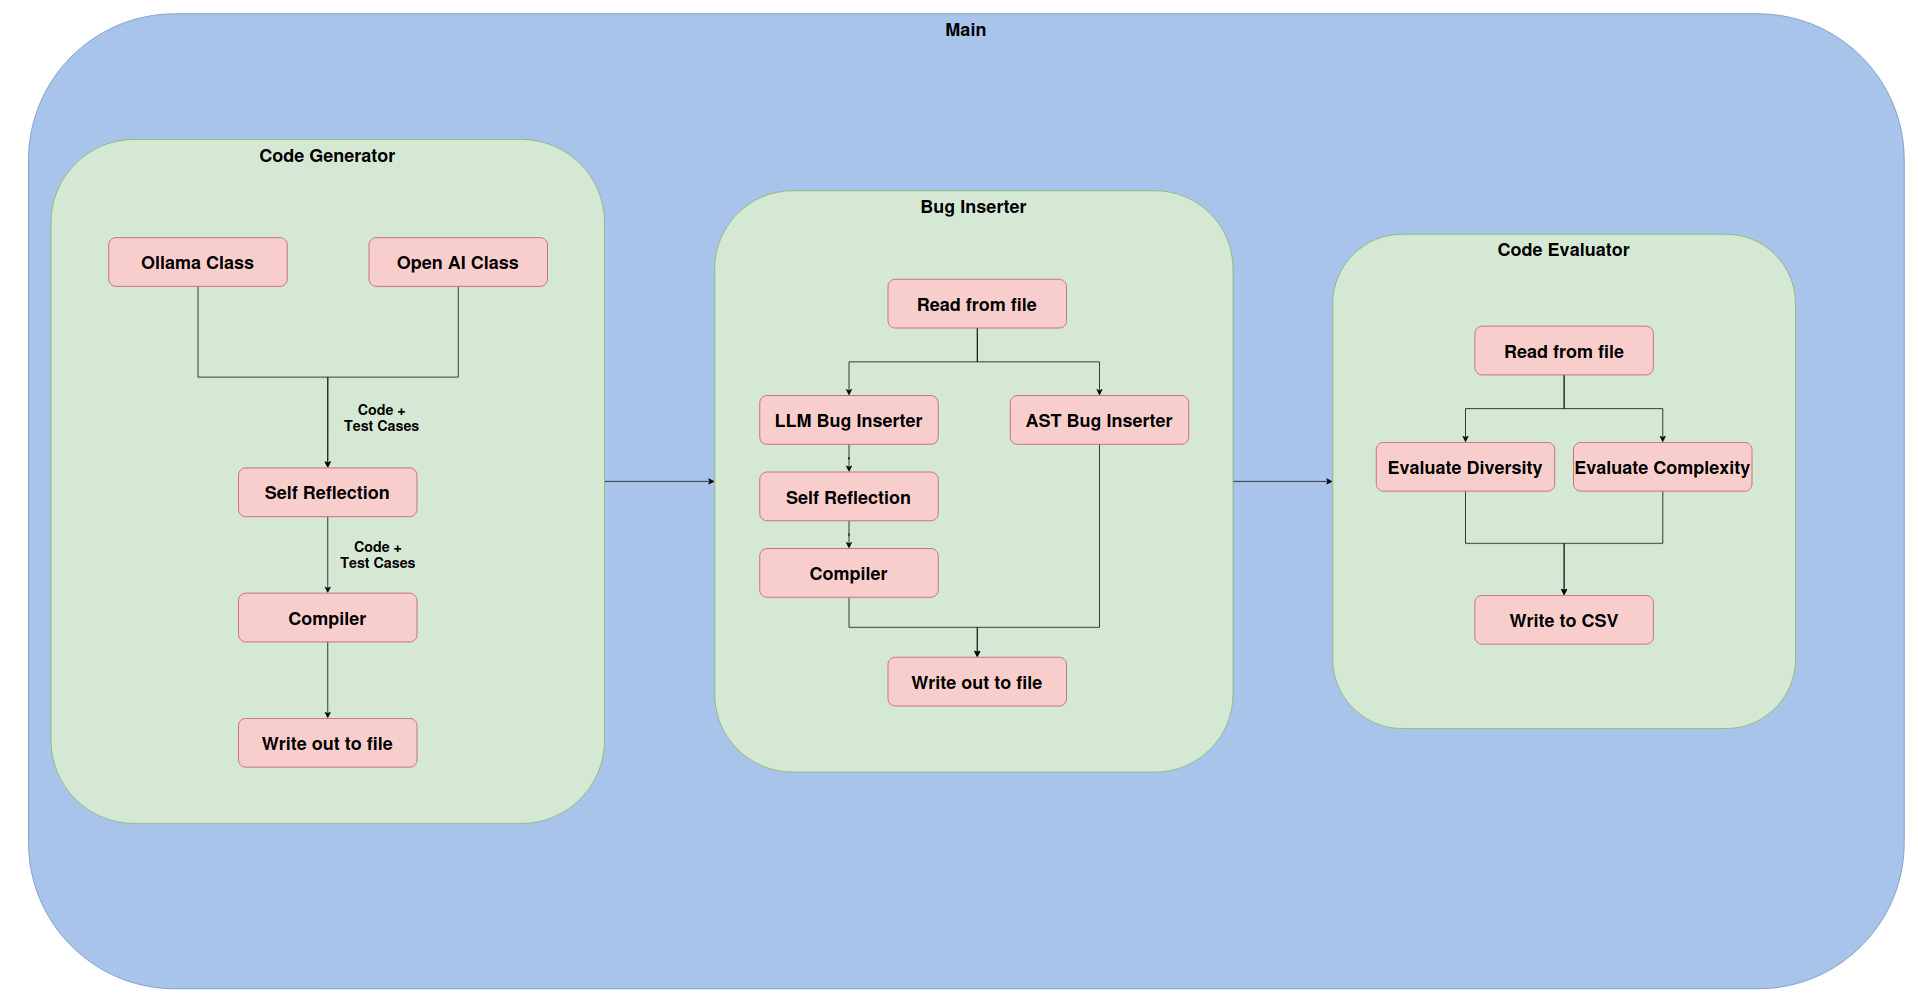
\includegraphics[width=\linewidth]{Images/Design.png}

The above diagram shows a pipeline diagram of the code. There is three main blocks to the code. The code generator which takes no input except for simple parameters such as model type and code topic. It will then produce functional code based on the topic mentioned. It will also ensure that the code is functional by compiling and checking for errors. 

The bug inserter will then take this working code and insert a bug into it, this is done by either the use of the LLM again or by using inspecting and altering the AST in the code. It will then check if the code now fails or produces the wrong output as it should do. This is only done for the LLM however as the AST bug inserter is not liable the same reliability issues of the LLM. This altered code is then written back out to the file overwriting the original code. The code evaluator will then take this code and run the diversity and complexity metrics on it before writing this to the csv.

\subsection{Tools}
\subsubsection{Ollama}

The first of the two major tools that was used in this project is ollama. This is a tool that facilitates easy interaction with LLMs running on a local machine. This tool allows for the usage of almost all popular models. This tool was downloaded by cloning the ollama repository from github and running the install script. Further models could then easily be pulled and run from command line using the following commands.

\begin{verbatim}
ollama pull <model>
ollama run <model>
<Interaction with LLM>
\end{verbatim}

This works perfectly well for interacting with the LLM like a chat bot but like this through some shell scripting language such as bash would not be the ideal solution. Fortunately the ollama API is much better suited to this task. The constructor for the class is called with some intialising hyperparameters and then a prompt can simple be passes to using the invoke method which returns the response from the LLM. This was then wrapped in a class for easy use in the project.

\subsubsection{OpenAI GPT API}

The process for using the OpenAI GPT API is a bit simpler since there is no setup but has a few more steps in the code for the protection of the API key. Due to this code being on a github repo and automated testing being done using github workflows there is a couple different environments that all need access to the API key. For the github workflow runner the key was stored as a secret and then passed to the code as an environment variable. For the local machine the key was stored in a file which was excluded from git commits using the .gitignore file. One this has been handled the interaction is very similar. The parameters, prompt and API key are passed to the constructor and then a function is called to get the response from the LLM.

\subsection{Code generation}

The code generation class is the first class called in the pipeline and is also the only class that interacts directly with the LLM. The class is called with the model type, file\_path and a number of different switches to enable different modes, the prompt is then adapted and phrased in a way that the code produced will always expect an input file called \texttt{input.txt}. The LLM is then called to generate the code and also generate the \texttt{input.txt} file. Both of these responses are then parsed and written to their respective files. The code is then run from a subprocess which will check if the code compiles and runs correctly. If the code does not compile or run correctly the function will return an error and the parent function will handle it. If it works correctly the function will return the response with the given \texttt{input.txt} which is used to determine later whether the bug inserter has worked correctly. Due to the input being in the format of a separate file it is very easy for multiple \texttt{input.txt} files to be generated and used as multiple different test cases. 
There is also an option for a prompt to be passed to the class which will override the original prompt. This is how the LLM bug insertion is able to interact with the LLM without creating duplicate logic. 

\subsubsection{Self Reflection \& Improvement}

As the project progressed it was clear that the local LLMs were having a lot of difficulty producing the correct code. This was very uncommmon with the openAI modules but to solve this self reflection and improvement was implemented in the code. 

As it became impossible to feed the LLMs more information in training a new technique emerged when developers would get the LLM to 'think' about their response. This is done by re-querying the LLM after it returns a response and asking it if the response it gave fits the original prompt. This process is called self reflection which is good for filtering out bad responses. Another similar method is called self improvement which is where the LLM is asked to improve on its response. This will attempt to fix bad responses and also attempt to improve already acceptable responses.

The issue that was noticed with this method was a significant increase in the runtime of the project. However it also meant that smaller modeuls could be used and provide better performance. It is not clear which method would be likely to yield a better response but the performance will be compared and discussed in the testing and evaluation section.

\subsection{Bug Insertion}
\subsubsection{LLM Bug Insertion}
\subsubsection{AST Bug Insertion}

\section{Testing and Evaluation}

This will discus the testing of the project which will show the improvement of the project over time. This will also include an evalution of the final state of the project.

\subsection{Environments}
\subsection{Benchmark Test Suite}
\subsection{Metrics}
\subsubsection{Code Complexity}
\subsubsection{Code Diversity}
\subsubsection{Attempt Count}
\subsubsection{Run Time}


\section{Conclusion}

This will briefly summarise the project and discuss the future of the project.

\newpage
\section{References}
\begin{thebibliography}{9}

\bibitem{jadud2006}
Jadud, M. C. (2006). Methods and tools for exploring novice compilation behaviour. Proceedings of the Second International Workshop on Computing Education Research, 73–84. https://doi.org/10.1145/1151588.1151600

\bibitem{li2019}
Li, C., Chan, E., Denny, P., Luxton-Reilly, A., \& Tempero, E. (2019). Towards a Framework for Teaching Debugging. Proceedings of the Twenty-First Australasian Computing Education Conference, 79–86. https://doi.org/10.1145/3286960.3286970

\bibitem{odell2017}
O’Dell, D. H. (2017). The Debugging Mindset: Understanding the psychology of learning strategies leads to effective problem-solving skills. Queue, 15(1), 71–90. https://doi.org/10.1145/3055301.3068754

\bibitem{parkinson2024}
Parkinson, M. M., Hermans, S., Gijbels, D., \& Dinsmore, D. L. (2024). Exploring debugging processes and regulation strategies during collaborative coding tasks among elementary and secondary students. Computer Science Education, 0(0), 1–28. https://doi.org/10.1080/08993408.2024.2305026

\bibitem{whalley2021}
Whalley, J., Settle, A., \& Luxton-Reilly, A. (2021). Analysis of a Process for Introductory Debugging. Proceedings of the 23rd Australasian Computing Education Conference, 11–20. https://doi.org/10.1145/3441636.3442300

\bibitem{whalley2023}
Whalley, J., Settle, A., \& Luxton-Reilly, A. (2023). A Think-Aloud Study of Novice Debugging. ACM Transactions on Computing Education, 23(2), 1–38. https://doi.org/10.1145/3589004

\bibitem{denny2023}
Denny, P., Leinonen, J., Prather, J., Luxton-Reilly, A., Amarouche, T., Becker, B. A., \& Reeves, B. N. (2023). Promptly: Using Prompt Problems to Teach Learners How to Effectively Utilize AI Code Generators. https://doi.org/10.48550/ARXIV.2307.16364

\bibitem{denny2024}
Denny, P., Leinonen, J., Prather, J., Luxton-Reilly, A., Amarouche, T., Becker, B. A., \& Reeves, B. N. (2024). Prompt Problems: A New Programming Exercise for the Generative AI Era. Proceedings of the 55th ACM Technical Symposium on Computer Science Education V. 1, 296–302. https://doi.org/10.1145/3626252.3630909

\bibitem{nguyen2024}
Nguyen, S., Babe, H. M., Zi, Y., Guha, A., Anderson, C. J., \& Feldman, M. Q. (2024). How Beginning Programmers and Code LLMs (Mis)read Each Other. Proceedings of the CHI Conference on Human Factors in Computing Systems, 1–26. https://doi.org/10.1145/3613904.3642706

\end{thebibliography}

\end{document}